\documentclass[screen, aspectratio=43,compress,dvipsnames]{beamer}
\usepackage[T1]{fontenc}
\usepackage[utf8]{inputenc}

\usepackage{textcomp}
\usepackage{lmodern}

\usepackage{tcolorbox}
\usepackage{booktabs}
\usepackage{array}
\usepackage{seqsplit}
\usepackage[absolute,overlay]{textpos}
\usepackage[normalem]{ulem}
\usepackage{xkeyval}
\usepackage{adjustbox}

\graphicspath{/build/}

\usepackage{tikz}
\usepackage[subpreambles,mode=image]{standalone}


\renewcommand\Longrightarrow{%
 \mathrel{%
  \mbox{\fontfamily{cmr}\fontencoding{OT1}\selectfont=}}%
 \joinrel\Rightarrow}


\newcount\mycount
\renewcommand\includestandalone[2][]{%
    \begingroup
    \pdfximage{#2.pdf}%
    \chardef\npages\pdflastximagepages\relax
    \mycount=1 %
    \loop
        \includegraphics<\the\mycount>[page=\mycount,#1]{#2.pdf}%
        \ifnum\mycount<\npages %
        \advance\mycount by 1 %
    \repeat
    \endgroup
}



\makeatletter
\let\beamer@writeslidentry@miniframeson=\beamer@writeslidentry
\def\beamer@writeslidentry@miniframesoff{%
  \expandafter\beamer@ifempty\expandafter{\beamer@framestartpage}{}% does not happen normally
  {%else
    % removed \addtocontents commands
    \clearpage\beamer@notesactions%
  }
}
\newcommand*{\miniframeson}{\let\beamer@writeslidentry=\beamer@writeslidentry@miniframeson}
\newcommand*{\miniframesoff}{\let\beamer@writeslidentry=\beamer@writeslidentry@miniframesoff}
\makeatother

\makeatletter
\newenvironment{inframe}[2][1]{%
  \edef\inframe@current{\the\value{beamerpauses}}%
  \setcounter{beamerpauses}{#1}%
  \beamer@slideinframe=#2\relax
  \let\beamer@anotherslidetrue=\@empty
  \let\beamer@localanotherslidetrue=\@empty
}{%
  \setcounter{beamerpauses}{\inframe@current}%
}

\newcommand{\vcenteredinclude}[1]{\begingroup
\setbox0=\hbox{#1}%
\parbox{\wd0}{\box0}\endgroup}

\newcommand\redout{\bgroup\markoverwith
{\textcolor{red}{\rule[0.5ex]{2pt}{1pt}}}\ULon}


\makeatother




\newcommand\FrameText[1]{%
  \begin{textblock*}{\paperwidth}(0.95\textwidth,0.5cm)
    \raggedright {#1}\hspace{.5em}
  \end{textblock*}
 }

\providecommand{\adlog}{\textcolor{red}{a}}
\providecommand{\bdlog}{\textcolor{blue}{b}}
\providecommand{\cdlog}{\textcolor{Plum}{c}}
\providecommand{\ddlog}{\textcolor{OliveGreen}{d}}
\providecommand{\dlog}[2]{\textcolor{#1}{#2}}
\providecommand{\ua}[1]{\dlog{red}{#1}}
\providecommand{\ub}[1]{\dlog{blue}{#1}}
\providecommand{\uc}[1]{\dlog{Plum}{#1}}
\providecommand{\ud}[1]{\dlog{OliveGreen}{#1}}

%\bibliography{../customrefs}
%\bibliographystyle{alpha}


\usetheme[style=horizontal,language=en]{ntnu2017}



\setbeamertemplate{itemize item}[circle]
\setbeamertemplate{itemize subitem}{--}

\title{Group key exchange}
\subtitle{Trial lecture}

\author{Håkon Jacobsen}
\institute{Department of Information Security and\\Communication Technology}
\date{October 25, 2017}




\begin{document}

\begin{frame}
  \titlepage
\end{frame}

% Alternatively, special title page command to get a different background
% \ntnutitlepage

\section{Intro}
\subsection{intro}




\begin{frame}<3>{Intro}
	\begin{figure}
		\centering
		\includestandalone[width=0.6\textwidth]{tikz_KE_motivation}
	\end{figure}
\end{frame}

%
\begin{frame}<4->{Key exchange protocols}
	\begin{figure}
		\includestandalone[width=0.6\textwidth]{tikz_KE_motivation}
	\end{figure}
	
%	\vspace*{-2em}
%	
%	\begin{itemize}
%		\item Key exchange protocols are everywhere 
%	\end{itemize}
\end{frame}


%\begin{frame}<1>[label=KE_example]{Example: IEEE 802.11 (Wi-Fi)}
%	\frametitle<2->{eduroam}
%	\begin{figure}
%		\includestandalone[width=0.75\textwidth]{tikz_intro_slide}
%	\end{figure}
%\end{frame}
%


\begin{frame}{Group key exchange}
	\begin{itemize}
		\item $N$ parties want to establish a shared session key for \textbf{group} communication
		
		\item[]

		\item Can encrypt message \textbf{once}  instead of $N$ times
		
		\item[]
		
		\item Many applications:
			\begin{itemize}
				\item group chats
				
				\item multi-device messaging
				
				\item video and audio conferencing
				
				\item TV broadcasting 
			\end{itemize}
		
		

	\end{itemize}
\end{frame}

%\begin{frame}{Group key exchange protocols}
%	\centering
%	\includestandalone[width=0.91\textwidth]{tikz_GKE_motivation}
%\end{frame}

\begin{frame}{Group key exchange goals}

	\begin{center}
		 \uncover<1->{
		 	\large $\mathcal{G} = \lbrace U_1, U_2, \dotsc, U_n \rbrace \quad$ 
			\vspace*{0.2cm}	
	
		}
	\end{center}
	
	\begin{itemize}
	
		\item<1-> \textbf{Correctness}: 
		all group members should derive the \emph{same} key $\ub{sk}$
			
		\item[]	
			
		\item<2-> \textbf{Key-secrecy}: 
		\uncover<1->{attacker should learn nothing about $\ub{sk}$}

		
		\item[]
		
		\item<3-> \textbf{Authentication}:
		\uncover<1->{agreement upon who the group members are
				
		(i.e., to whom $\ub{sk}$ is shared with)
		}	 

	
	\end{itemize}
\end{frame}


\begin{frame}{Special challenges in \emph{group} key exchange}
	\begin{itemize}
			
		\item Dynamic groups 
			\begin{itemize}
				\item user might \textbf{join} already existing group 
				
				\item user might \textbf{leave} current group
			\end{itemize}
		
		\item[]

		\item Malicious group members / insider attacks
			\begin{itemize}
				\item can trivially learn session key $sk$ 
				
				\item but may also be able to impersonate \textbf{other honest} users of the group, 
				or  make honest users agree upon different keys
			
				\item collusion among several insiders
			\end{itemize}
	
		\item[]
		
		\item Efficiency considerations
	
	\end{itemize}

\end{frame}


\begin{frame}{Complexity measures for group key exchange}
	\begin{itemize}
		\item  Round complexity
		\begin{itemize}
			\item latency 
		\end{itemize}
		
		\item[]
		
		\item Communication complexity
		\begin{itemize}
			\item number of messages sent 
			\item point-to-point links vs broadcast channels
		\end{itemize}
		
		\item[]
		
		\item Computational complexity
	\end{itemize}
\end{frame}



\section{Group KE}
\subsection{group KE}






\begin{frame}<1-12>{Diffie-Hellman key exchange}
	
	Fix a \emph{large} prime $p$
	
	Fix an integer $g$ in $\lbrace 1, 2, \dotsc, p - 1 \rbrace$

	\begin{figure}
		\centering
%		\fbox{%
			\includestandalone[trim={1cm 3.5cm 1cm 2.4cm},clip,width=0.99\textwidth]{tikz_DH}
%		}
	\end{figure}
	
	
	\visible<4->{
		\begin{tikzpicture}[remember picture,overlay]
		    \node[xshift=-2cm,yshift=-1.65cm] at (current page.north east) {\includegraphics[width=0.28\textwidth]{tikz_circle}};
		\end{tikzpicture}
	}
	

	\uncover<9->{

		\textbf{Security}

		Attacker sees: $p$, $g$,  $g^{\adlog}$, $g^{\bdlog}$
	
		Can the attacker compute $g^{\adlog\bdlog}$? \uncover<10->{Can compute $g^{\adlog} \cdot g^{\bdlog} = g^{\adlog + \bdlog}$ }
	}
	
	\visible<11->{
		\begin{tikzpicture}[remember picture,overlay]
   			\node[xshift=-4cm,yshift=3.2cm,draw=red,thick,fill=lightgray!20,align=left,inner sep=0.2cm] at (current page.south east) {
   				Assumptions for the rest of this talk:\\
   				$\ $1. \textbf{impossible} to compute $g^{\adlog\bdlog}$ from $g^{\adlog}$, $g^{\bdlog}$\\
   				$\ $2. \textbf{impossible} to compute $\ua{x}$ from $g^{\ua{x}}$
   			};
		\end{tikzpicture}
	}

	\uncover<12->{
		\begin{tikzpicture}[remember picture,overlay]
		    \node[xshift=0cm,yshift=0.75cm,font=\tiny,align=left,fill=white,inner ysep=0.4cm] at (current page) {%
		    	\parbox{\linewidth}{
		    	$p = \seqsplit{%
		    			323170060713110073003389139264238282488179412411402391128420097514007417066343542226196894173635693471179017379097041917
		    			546058732091950288537589861856221532121754125149017745202702357960782362488842461894775876411059286460994117232454266225
		    			221932305409190376805242355191256797158701170010580558776510388618472802579760549035697325615261670813393617995413364765
		    			591603683178967290731783845896806396719009772021941686472258710314113364293195361934716365332097170774482279885885653692
		    			086452966360772502689555059283627511211740969729980684105543595848665832916421362182310789909994486524682624169720359118
		    			52507045361090559}$	
		    	}
		    };
		\end{tikzpicture}
	}

\end{frame}

%\begin{frame}{Diffie-Hellman key exchange -- Man-in-the-Middle attack}
%	\begin{figure}
%		\centering
%%		\fbox{%
%			\includestandalone[trim={1cm 3cm 1cm 2cm},clip,width=0.9\textwidth]{tikz_DH_MitM}
%%		}
%	\end{figure}
%\end{frame}






\begin{frame}{Protocol 1 -- Ingemarsson, Tang, \& Wong (1982) \nocite{IngemarssonTW:1982}}
	\newcommand{\wheelwidth}{0.9} %
	\newcommand{\wheelcolwidth}{0.33} %
	\newcommand{\settrimming}{%
	    \setkeys{Gin}{%
	        trim = 2.2cm 2cm 3.3cm 1cm,clip=true,
	        width=\textwidth,
	    }
	    \presetkeys{Gin}{clip}{}
	}
	\settrimming
	\begin{columns}
		\hspace*{0.5cm}
		\centering
		\begin{column}{\wheelcolwidth\textwidth}
			\begin{overlayarea}{\textwidth}{4cm}
				\only<1-2>{
					\includegraphics[page=1,width=\wheelwidth\textwidth]{tikz_protocol_Ingemar}
				}
				\only<3-6>{
					\includegraphics[page=2,width=\wheelwidth\textwidth]{tikz_protocol_Ingemar}
				}
				\only<7->{
					\includegraphics[page=5,width=\wheelwidth\textwidth]{tikz_protocol_Ingemar}
				}
			\end{overlayarea}
		\end{column}
		\hspace*{-0.0cm}
		\begin{column}{\wheelcolwidth\textwidth}
			\begin{overlayarea}{\textwidth}{4cm}
				\only<4-6>{
					\includegraphics[page=3,width=\wheelwidth\textwidth]{tikz_protocol_Ingemar}
				}
				\only<7->{
					\includegraphics[page=6,width=\wheelwidth\textwidth]{tikz_protocol_Ingemar}
				}
			\end{overlayarea}
		\end{column}
		\hspace*{-0.0cm}
		\begin{column}{\wheelcolwidth\textwidth}
			\begin{overlayarea}{\textwidth}{4cm}	
				\only<5-6>{
					\includegraphics[page=4,width=\wheelwidth\textwidth]{tikz_protocol_Ingemar}
				}
				\only<7->{
					\includegraphics[page=7,width=\wheelwidth\textwidth]{tikz_protocol_Ingemar}
				}
			\end{overlayarea}
		\end{column}
	\end{columns}
	\begin{columns}
		\begin{column}{0.6\textwidth}
			\small
			\uncover<2->{Goal: compute $sk \gets g^{\adlog\bdlog\cdlog\ddlog}$}
					
			\uncover<9->{%
				\begin{tabbing}
					\textbf{Security:}\\
					Attacker sees: \= $g^{\adlog}, g^{\bdlog}, g^{\cdlog}, g^{\ddlog}$\\
					\> $g^{\adlog\bdlog}, g^{\bdlog\cdlog}, g^{\cdlog\ddlog}, g^{\adlog\ddlog}$ \\
					\> $g^{\adlog\bdlog\cdlog}, g^{\adlog\bdlog\ddlog}, g^{\adlog\cdlog\ddlog}, g^{\bdlog\cdlog\ddlog}$
				\end{tabbing}				
			}
		\end{column}

		\begin{column}{0.4\textwidth}
			\begin{itemize}[]
				\small{
				\item<8->[] \textcolor{red}{$A$}:  $sk \gets (g^{\bdlog\cdlog\ddlog})^{\adlog}$
				
				\item<8->[] \textcolor{blue}{$B$}:  $sk \gets (g^{\adlog\cdlog\ddlog})^{\bdlog}$
				
				\item<8->[] \textcolor{Plum}{$C$}:  $sk \gets (g^{\adlog\bdlog\ddlog})^{\cdlog}$
				
		 		\item<6->[] \textcolor{OliveGreen}{$D$}:  $sk \gets (g^{\adlog\bdlog\cdlog})^{\ddlog}$
		 		
		 		\item[]
		 		}
			\end{itemize}
		\end{column}
	
	\end{columns}

\end{frame}







%\begin{frame}{Protocol 2 -- Steiner, Tsudik, \& Waidner (1996) \nocite{CCS:SteTsuWai96}}
%%
%	\begin{figure}
%		\centering
%%		\vspace*{-1cm}
%%		\fbox{
%			\includestandalone[trim={1cm 2cm 1cm 1.4cm},clip,width=0.8\textwidth]{tikz_protocol_GDH1}
%%		}
%	\end{figure}
%	%
%	
%
%	Goal: compute $sk \gets g^{\adlog\bdlog\cdlog\ddlog}$
%%
%\end{frame}




\begin{frame}{Protocol 2 -- Kim, Perrig, \& Tsudik (2000) \nocite{CCS:KimPerTsu00}}

	\begin{figure}
		\centering
		\includestandalone[trim={0 1cm 0 0},clip,width=0.7\textwidth]{tikz_protocol_tree}
	\end{figure}
	
	\uncover<4->{$sk = \dlog{PineGreen}{z}$}
	
\end{frame}



\begin{frame}{Protocol 3 -- Burmester \& Desmedt (1994) \nocite{EC:BurDes94}}

	\vspace*{-1cm}
	\begin{figure}
		\centering
		\hspace*{1.2cm}
		\includestandalone[trim={1.2cm 2.2cm 1.1cm 1.5cm},clip,width=0.9\textwidth]{tikz_protocol_BDB}
	\end{figure}
	
	Goal: compute $sk \gets g^{\adlog\bdlog + \bdlog\cdlog + \cdlog\ddlog + \adlog\ddlog}$ 
	
\end{frame}



\begin{frame}{Protocol comparisons -- complexity}
	\centering
	\begin{tabular}{m{3cm} c >{\centering\arraybackslash}p{2.2cm} c}
			
		& Rounds & Messages & Exponentiations \\
		
		\cmidrule{2-4}
			
		\makebox[3.1cm][c]{\includegraphics[page=3,trim={0 2cm 0 1cm},clip,width=0.17\textwidth]{tikz_protocol_Ingemar}} & $N-1$ & $N-1$ & $N$ \\
%		\includegraphics[page=7,trim={0 2.2cm 0 0},clip,width=0.24\textwidth]{tikz_protocol_GDH1} & $2 ( N - 1)$ & $1$ & $i + 1$ \\
		\makebox[2.9cm][c]{\includegraphics[page=3,trim={0 0 0 0},clip,width=0.17\textwidth]{tikz_protocol_tree}} & $\log_2 N$ & $N - 1$  & $\log_2 N$ \\		
		\includegraphics[page=8,trim={0 1.9cm 0 30pt},clip,width=0.29\textwidth]{tikz_protocol_BDB} & 2 & $2(N - 1)$ & $\approx 3$ \\
	\end{tabular}
\end{frame}


\begin{frame}{Does there exist a 1-round $N$-party Diffie-Hellman protocol?}
	\begin{itemize}
		\item<2-> $N = 2$: standard 2-party Diffie-Hellman
		
		
		\item[] 
		
		\item<3-> $N = 3$: possible based on \textbf{bilinear pairings} (Joux 2000) \nocite{JC:Joux04}		
		
		
		\item[] 
		
		
		\item<4-> $N = 4, 5, 6 \dotsc$ \hspace*{0.3cm}\uncover<5->{\textbf{open problem}}
	\end{itemize}
\end{frame}







\section{Authentication}
\subsection{group ake}


\miniframesoff
\begin{frame}
	\usebeamerfont*{frametitle} 
	\usebeamercolor[fg]{frametitle}
	
	\vfill
	\vfill
	\vfill
	\centering
	Authenticated group key exchange
	\vfill
	\vfill
	\vfill
\end{frame}
\miniframeson


\begin{frame}{Authentication challenges}

	\begin{itemize}			
		\item Want to protect against \textbf{active} attackers
	
		\item[]
		
		\item Attacker should not be able to modify messages undetected
		
		\item[]
	
		\item Malicious group members / insider attacks
		
	\end{itemize}
\end{frame}

\begin{frame}{Katz \& Yung compiler (2003) \nocite{C:KatYun03}}
	
	\begin{itemize}
		\item Generic transformation
		
		\item[]
		
		\item \textbf{Passively} secure group KE $\implies$ \textbf{actively} secure group KE 
		
		\item[]
		
		\item Ingredients: \textbf{unique numbers} (nonces) + \textbf{digital signatures} 
	\end{itemize}
	
\end{frame}

\begin{frame}<1-5>{Protocol 1 + Katz \& Yung compiler}
	
	\vspace*{-0.5cm}
	\begin{columns}
		\hspace*{0.5cm}
		\begin{column}{0.33\textwidth}
			\uncover<5>{{\footnotesize Additional cost:
				\begin{itemize}
				\item 1 extra round
				\item $N - 1$ signatures
				\item $N - 1$ verifications
				\end{itemize}
				}
			}
		\end{column}
		\begin{column}{0.33\textwidth}
			\uncover<2->{
				\hspace*{0.5pt}
				\includegraphics[width=1.3\textwidth]{tikz_protocol_Ingemar_KY_broadcast}
			}
		\end{column}
		\begin{column}{0.33\textwidth}
			\uncover<3->{\hspace*{0.7cm}\mbox{\footnotesize$R \gets \ua{R_A} || \ub{R_B} || \uc{R_C} || \ud{R_D}$}}
		\end{column}
	\end{columns}
	\vspace*{-0.55cm}
	\begin{columns}
		\begin{column}{0.33\textwidth}
			\begin{overlayarea}{\textwidth}{3cm}
				\only<1-3>{
					\includestandalone[page=2,width=1.2\textwidth]{tikz_protocol_Ingemar}
				}
				\only<4->{
					\includestandalone[page=8,width=1.2\textwidth]{tikz_protocol_Ingemar}
				}
			\end{overlayarea}
		\end{column}
		\begin{column}{0.33\textwidth}
			\begin{overlayarea}{\textwidth}{3cm}
				\only<1-3>{
					\includestandalone[page=3,width=1.2\textwidth]{tikz_protocol_Ingemar}
				}
				\only<4->{
					\includestandalone[page=9,width=1.2\textwidth]{tikz_protocol_Ingemar}
				}
			\end{overlayarea}
		\end{column}
		\begin{column}{0.33\textwidth}
			\begin{overlayarea}{\textwidth}{3cm}
				\only<1-3>{
					\includestandalone[page=4,width=1.2\textwidth]{tikz_protocol_Ingemar}
				}
				\only<4->{
					\includestandalone[page=10,width=1.2\textwidth]{tikz_protocol_Ingemar}
				}
			\end{overlayarea}
		\end{column}		
	\end{columns}
	
	\bigskip
	
	\hfill \footnotesize$\ud{D} : sk \gets (g^{\adlog\bdlog\cdlog})^{\ddlog}$
\end{frame}

%%\begin{frame}{Gao, Neupane, \& Steinwandt (2014)\\
%% (Bohli, Gonzalez Vasco, \& Steinwandt (2007))}
%%
%%
%%	\begin{figure}
%%		\centering
%%		\includestandalone[width=0.93\textwidth]{tikz_protocol_Bohli}
%%	\end{figure}
%%	
%%\end{frame}


\section{Group messaging}
\subsection{group messaging}


\miniframesoff
\begin{frame}
	\usebeamerfont*{frametitle} 
	\usebeamercolor[fg]{frametitle}
	
	\vfill
	\vfill
	\vfill
	\centering
	Group text messaging
	\vfill
	\vfill
	\vfill
\end{frame}
\miniframeson



\begin{frame}{Group text messaging}

	\begin{columns}
	
		\begin{column}{0.7\textwidth}
			\begin{itemize}
				\item Very popular
						
	
				\item[] \vcenteredinclude{
\includegraphics[width=0.08\textwidth]{whatsapp_logo}} WhatsApp
				
				\item[] \vcenteredinclude{
\includegraphics[width=0.07\textwidth]{messenger_logo}} \alt<3->{\redout{Messenger}}{Messenger} \uncover<4->{Secret Conversations}
				
				\item[] \vcenteredinclude{
\includegraphics[width=0.08\textwidth]{signal_logo}} Signal
	
				\item[] \vcenteredinclude{
\includegraphics[width=0.075\textwidth]{imessage_logo}} \alt<2->{\redout{iMessage}}{iMessage}
				
				\item[] \vcenteredinclude{
\includegraphics[width=0.072\textwidth]{threema_logo}} \alt<2->{\redout{Threema}}{Threema}
	
				\item[]
	
				\item \textbf{Asynchronous} communication
				
				\item[]
				
				\item[]

				
			\end{itemize}
		\end{column}	
		\begin{column}{0.3\textwidth}
			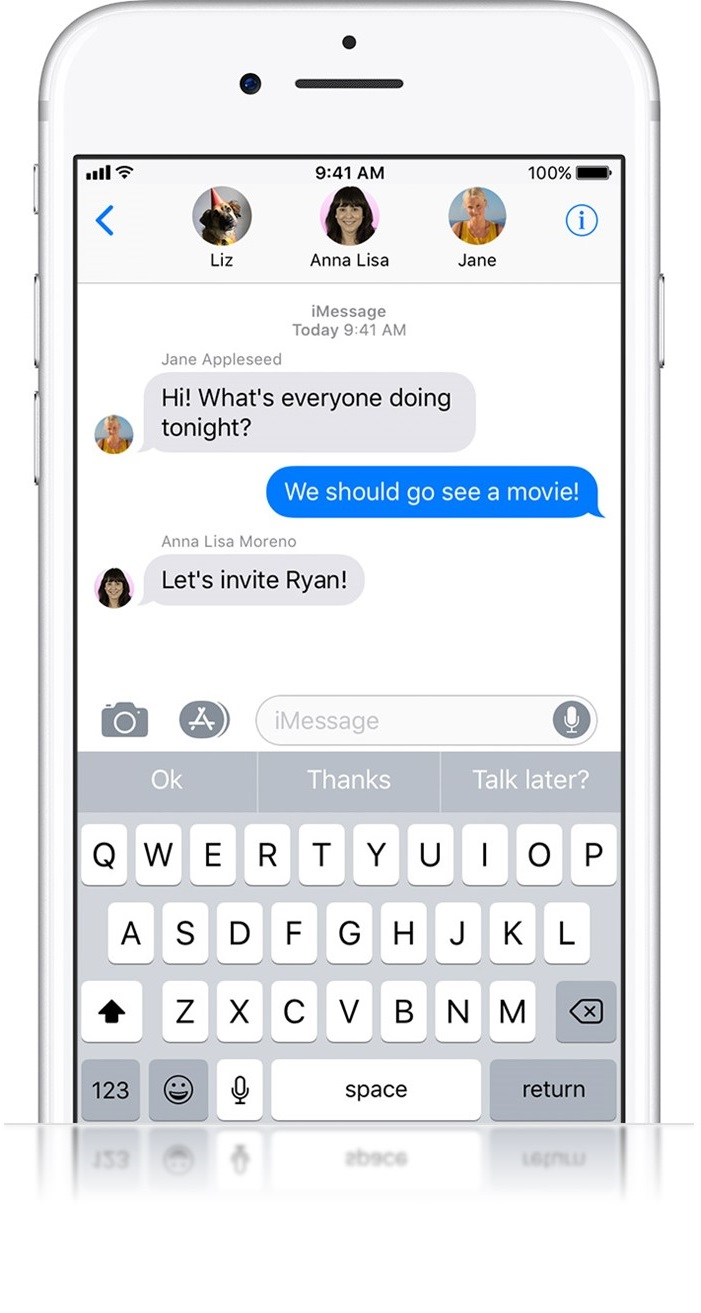
\includegraphics[width=1\textwidth]{imessage_group_chat2}
		\end{column}

	\end{columns}
	
\end{frame}

\begin{frame}{Sender Keys}

	\begin{itemize}
		
		\item Each user distributes personal group key (\textbf{Sender Key}) to each user in group
		over pairwise channel 
		
		\item[]
		
		\item Uses \textbf{pre-keys} to solve the asynchronous problem 
		
		\item[]
			
		\item Sender Key is \textbf{ratcheted} forward for each message sent 
		
		
		\item[]
		
		\item User \textbf{joins} group $\implies$ ratchet key forward
		
		\item[]
		
		\item User \textbf{leaves} group $\implies$ run protocol again
		
	\end{itemize}


\end{frame}

\begin{frame}{Asynchronous Ratcheting Tree (ART) -- Cohn-Gordon, Cremers, Garrat, Millican, \& Milner (2017) \nocite{EPRINT:CCGMM17}}
	\begin{itemize}
		\item Proposed Signal-like group key exchange protocol
		
		\item[]
		
		\item Based on tree structure
		
		\item[] 
		
		\item Achieves \textbf{post-compromise} security (like 2-party Signal)
	\end{itemize}
\end{frame}


%\begin{frame}{Sender Keys}
%
%	\begin{figure}
%		\centering
%		\hspace*{1cm}
%		\includestandalone[width=0.85\textwidth]{tikz_protocol_SenderKeys}
%	\end{figure}
%
%\end{frame}



\section{}


\begin{frame}{The End}
	\begin{center}
		Thank you
	\end{center}
\end{frame}


\bibliography{../customrefs,../cryptobib/abbrev3,../cryptobib/crypto}
\bibliographystyle{alpha}

\end{document}